\chapter{Generative Adversarial Networks - Implémentation}

 La structure théorique des \textbf{Generative Adversarial Networks} étant maintenant définie, nous devons implémenter ces réseaux. Pour cela, nous nous sommes lancés dans la continuité de MNIST, avec la génération de chiffres manuscrits par le \textbf{Générateur}, qui doit alors convaincre le \textbf{Discriminateur}. Ce cas de figure est idéal pour une première implémentation des GAN, puisque nous restons avec des données relativement simple (Dimension 28*28, en niveau de gris), avec un format normalisé et une importante base de données à disposition (La base de données MNIST : 60000 images d'apprentissages, 10000 données de test).

Le \textbf{Discriminateur} s'entraine donc à reconnaître les chiffres provenant de la base de données de MNIST en les différenciant des chiffres factices créés par le \textbf{Générateur}. Dans un premier temps, nous travaillons sur des chiffres uniques, en apprenant au Discriminateur à reconnaitre uniquement de 3 par exemple.

Nous verrons dans ce chapitre tout d'abord l'implémentation de notre GAN, puis les premiers résultats obtenus. Ces résultats nous ont confronté à divers problèmes, que nous aborderons alors avec les différentes solutions envisagées.


\section{Implémentation des \textit{Generative Adversarial Networks}}
\subsection{Présentation de la structure}
\subsection{Ratio d'apprentissage}

\section{Premiers résultats}

\section{Difficultés rencontrées et solutions émises}

Au cours du développement des GANs, nous avons été confrontés à de très nombreuses difficultés, que nous avons tenté de répertorier avec les solutions envisagées. À l'heure actuelle, certains problèmes sont toujours sans solution probante et restent des domaines de recherches ouverts : c'est le cas en particulier du \textbf{mode collapse} que nous détaillons ci-après.

\subsection{Le problème d'évaluation des performances}

Le premier et plus grand problème que nous avons rencontré est \textbf{l'absence de méthode systématique d'évaluation des performances d'un réseau donné.}

En effet, pour qu'un protocol expérimental puisse être mené à bien, il faut comparer un résultat témoin avec les résultats pour lesquels des paramètres ont varié, et déduire de la différence des performances si le paramètre testé est signifiant, et dans quelle mesure.

Ce protocole est \textbf{fondamental} en recherche expérimentale, et il est \textbf{inapplicable} ici. En effet, nous n'avons trouvé aucun moyen de mesurer la qualité d'une image, à l'exception de la mesure à l'oeil par les membres de l'équipe (ce qui ne peut être qualifié de méthode rigoureuse et systématique d'évaluation). 

\subsubsection{Les données à disposition pour mesurer les performances}

Afin de bien cerner le problème, résumons ce que nous avons à disposition à la fin d'une expérience. Si dans certains cas nous avons fait des essais nous permettant de mesurer d'autres grandeurs que les suivantes (comme la valeur des poids etc), seules les deux ci-après sont accessibles systématiquement, pour chaque expérience.
Nous disposons donc de :

\begin{itemize}
  \item Un ensemble d'images de synthèse générées à différents instants d'apprentissage; par exemple nous pouvons demander à produire 100 images tous les 10 apprentissages, ce qui permet de suivre assez finement l'évolution du GAN au fur et à mesure de son apprentissage
  \item Les courbes de score des deux réseaux, générées à la fin de l'expérience. La courbe de score d'un réseau représente la proportion d'erreurs dans toutes les réponses qu'il donne. Ainsi la courbe de score du discriminateur compte le nombre de bonnes réponses du réseau à des entrées aussi bien de synthèse (réponse attendue : 0) que réelles (réponse attendue : 1); la courbe du générateur est calculée en fonction des réponses du discriminateur aux images de synthèse. Ces courbes sont graduées en abscisse par rapport à nombre d'apprentissages effectués.
\end{itemize}

\subsubsection{Évaluation par réseau(x) tiers}

Une première idée pour l'évaluation, serait de passer les images de synthèses dans un 3ème réseau (appelons le évaluateur, mais il se comporte exactement comme le discriminateur) qui aurait appris à part, en dehors de la structure de GAN et qui serait un juge objectif sur les résultats du GAN. Ce réseau aurait été entraîné sur les données réelles, et resterait immuable une fois son apprentissage terminé. 

Cette méthode est en pratique inapplicable (et inappliquée, pour ce que nous en savons), notamment à cause de la difficulté à équilibrer ce 3ème réseau avec les deux autres; équilibrer un GAN est déjà une tâche particulièrement ardue (nous y reviendrons), ajouter cet évaluateur la rend insurmontable. Car si l'évaluateur est très performant, il risque de donner une performance nulle à tous les générateurs qu'il testera; à l'inverse si on l'a délibérément fait peu apprendre, il ne permettra pas de discriminer efficacement les générateurs qu'il testera.

On pourrait envisager de créer une échelle d'évaluateurs, constituée de plusieurs évaluateurs ayant chacun arrêté leur apprentissage à un moment différent, afin de pouvoir graduer les résultats obtenus par les générateurs sur une échelle de performance. Nous n'avons pas nous même implémenté cette technique et n'avons pas trouvé d'articles faisant mention de l'application de cette méthode, mais elle a au moins l'avantage majeur d'être rigoureuse, systématique et indépendante du jugement humain.

\subsection{Mode Collapse du \textit{Generateur} vers un unique point}
\subsubsection{Présentation du problème}

Un problème récurrent que l'on peut observer dans les GAN est le \textit{mode collapse}, ou \textit{missing modes}. Prenons un GAN, le générateur doit tenter de créer des images les plus réalistes possible par rapport à une distribution de données réelles, par l'intermédiaire du discriminateur. Cette distribution peut présenter plusieurs modes, plusieurs zones en quelque sorte (En reprenant l'exemple des chiffres de MNIST, on peut vouloir générer des 3, ou des 4). 
Cependant, on observe que le générateur a souvent tendance à apprendre à ne générer qu'un seul mode. On appelle cela le mode collapse : le générateur apprendra à aller vers une des zones de la distribution voulue, se rendra compte que cette zone marche, et y restera. 
Sur l'exemple simplifié ci-dessous, la distribution d'origine présente 4 zones, et le GAN n'en couvre qu'une seule. 

\begin{figure}[h]
\begin{center}
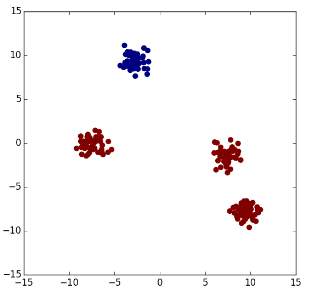
\includegraphics[width=0.5\textwidth]{images/missing_modes.png}\caption{Missing modes : les points répresentent les éléments de la distribution de donnéees réelles. En bleu l'ensemble de sortie du GAN appartenant à la distribution réelle, et en rouge les zones de la distribution initiale non couverte par le GAN.}
\end{center}
\end{figure} 

Ce phénomène récurrent est observable à différents degrés : on peut avoir des collapses partiels, les données générées seront donc variables mais toute la distribution ne sera pas représentée par le générateur, ou des collapses totaux, où le générateur ne sera qu'une projection vers un point. Les données générées seront alors très proches les unes des autres.
Nous avons été confrontés à ce problème de collapse total en générant des chiffres à partir de la base de données MNIST. Comme montré ci-dessous, en essayant de générer des 3, nous obtenons pour un réseau donné, des images générées qui sont toutes très proches, avec la même forme de 3, les mêmes pixels singuliers.

\begin{figure}[h]
\begin{center}
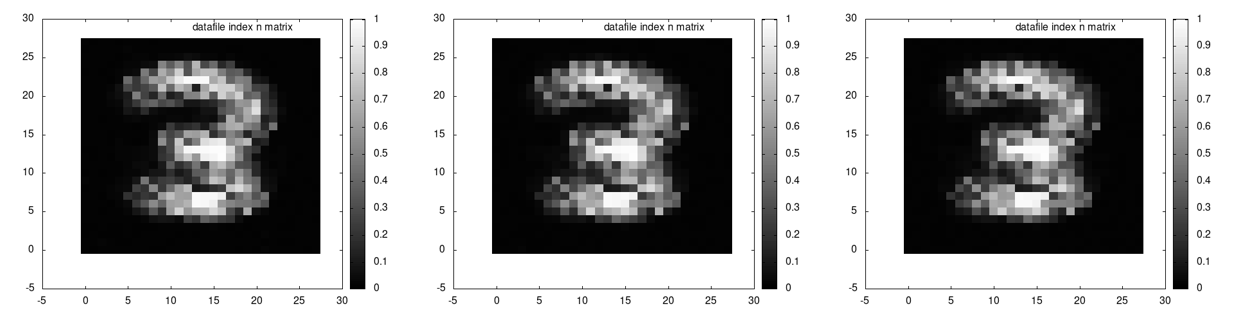
\includegraphics[width=1\textwidth]{images/missing_modes_2.png}\caption{Missing modes : On obtient pour un même réseau, 3 échantillons générés qui sont sensiblement les mêmes.}
\end{center}
\end{figure}


\subsubsection{Solution envisagée : Retrait du biais dans les réseaux (non fructueuse)}

Une première hypothèse concernant ce problème de Mode Collapse était la suivante : l'unique image produite par le générateur n'était en réalité qu'une image du masque de biais qui figeait l'image, par exemple en plaçant certains biais trop haut ou trop bas, annulant les entrées bruitées en début de réseau. On aurait alors une image déterminée uniquement par les biais, ce qui expliquerait un collapse vers une unique image.
De plus, en observant précisément le masque de biais sous forme matricielle, on remarque que ses poids forment effectivement l'image d'un nombre, comme on peut le voir ci-dessous :

\begin{figure}[h]
\begin{center}
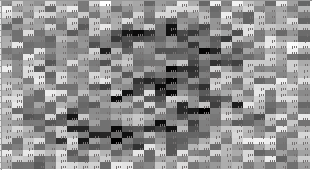
\includegraphics[width=0.5\textwidth]{images/masqueBiais.png}\caption{Masque du biais : on peut observer que le biais forme lui même les bases d'une image, un 3 ici.}
\end{center}
\end{figure}

On peut vérifier cette supposition en supprimant les biais de nos réseaux de neurones. On aurait alors plus de valeurs constantes qui figeraient l'image. Cependant, en implémentant ces réseaux, on n'observe qu'un ralentissement de l'apprentissage vers un état de Collapse similaire : les résultats sont moins intéressants (chiffres moins beaux), l'apprentissage est plus lent, et on converge toujours vers un Mode Collapse.

La suppression du biais ne permet donc pas de résoudre ce problème, c'est bien la fonction de transfert globale du réseau de neurones qui converge vers cet unique point.  


\subsubsection{Solution envisagée : Injection de bruit dans chaque couche du Générateur (fructueuse)}
